\label{scenario}
\begin{figure}[t]
	\centering
	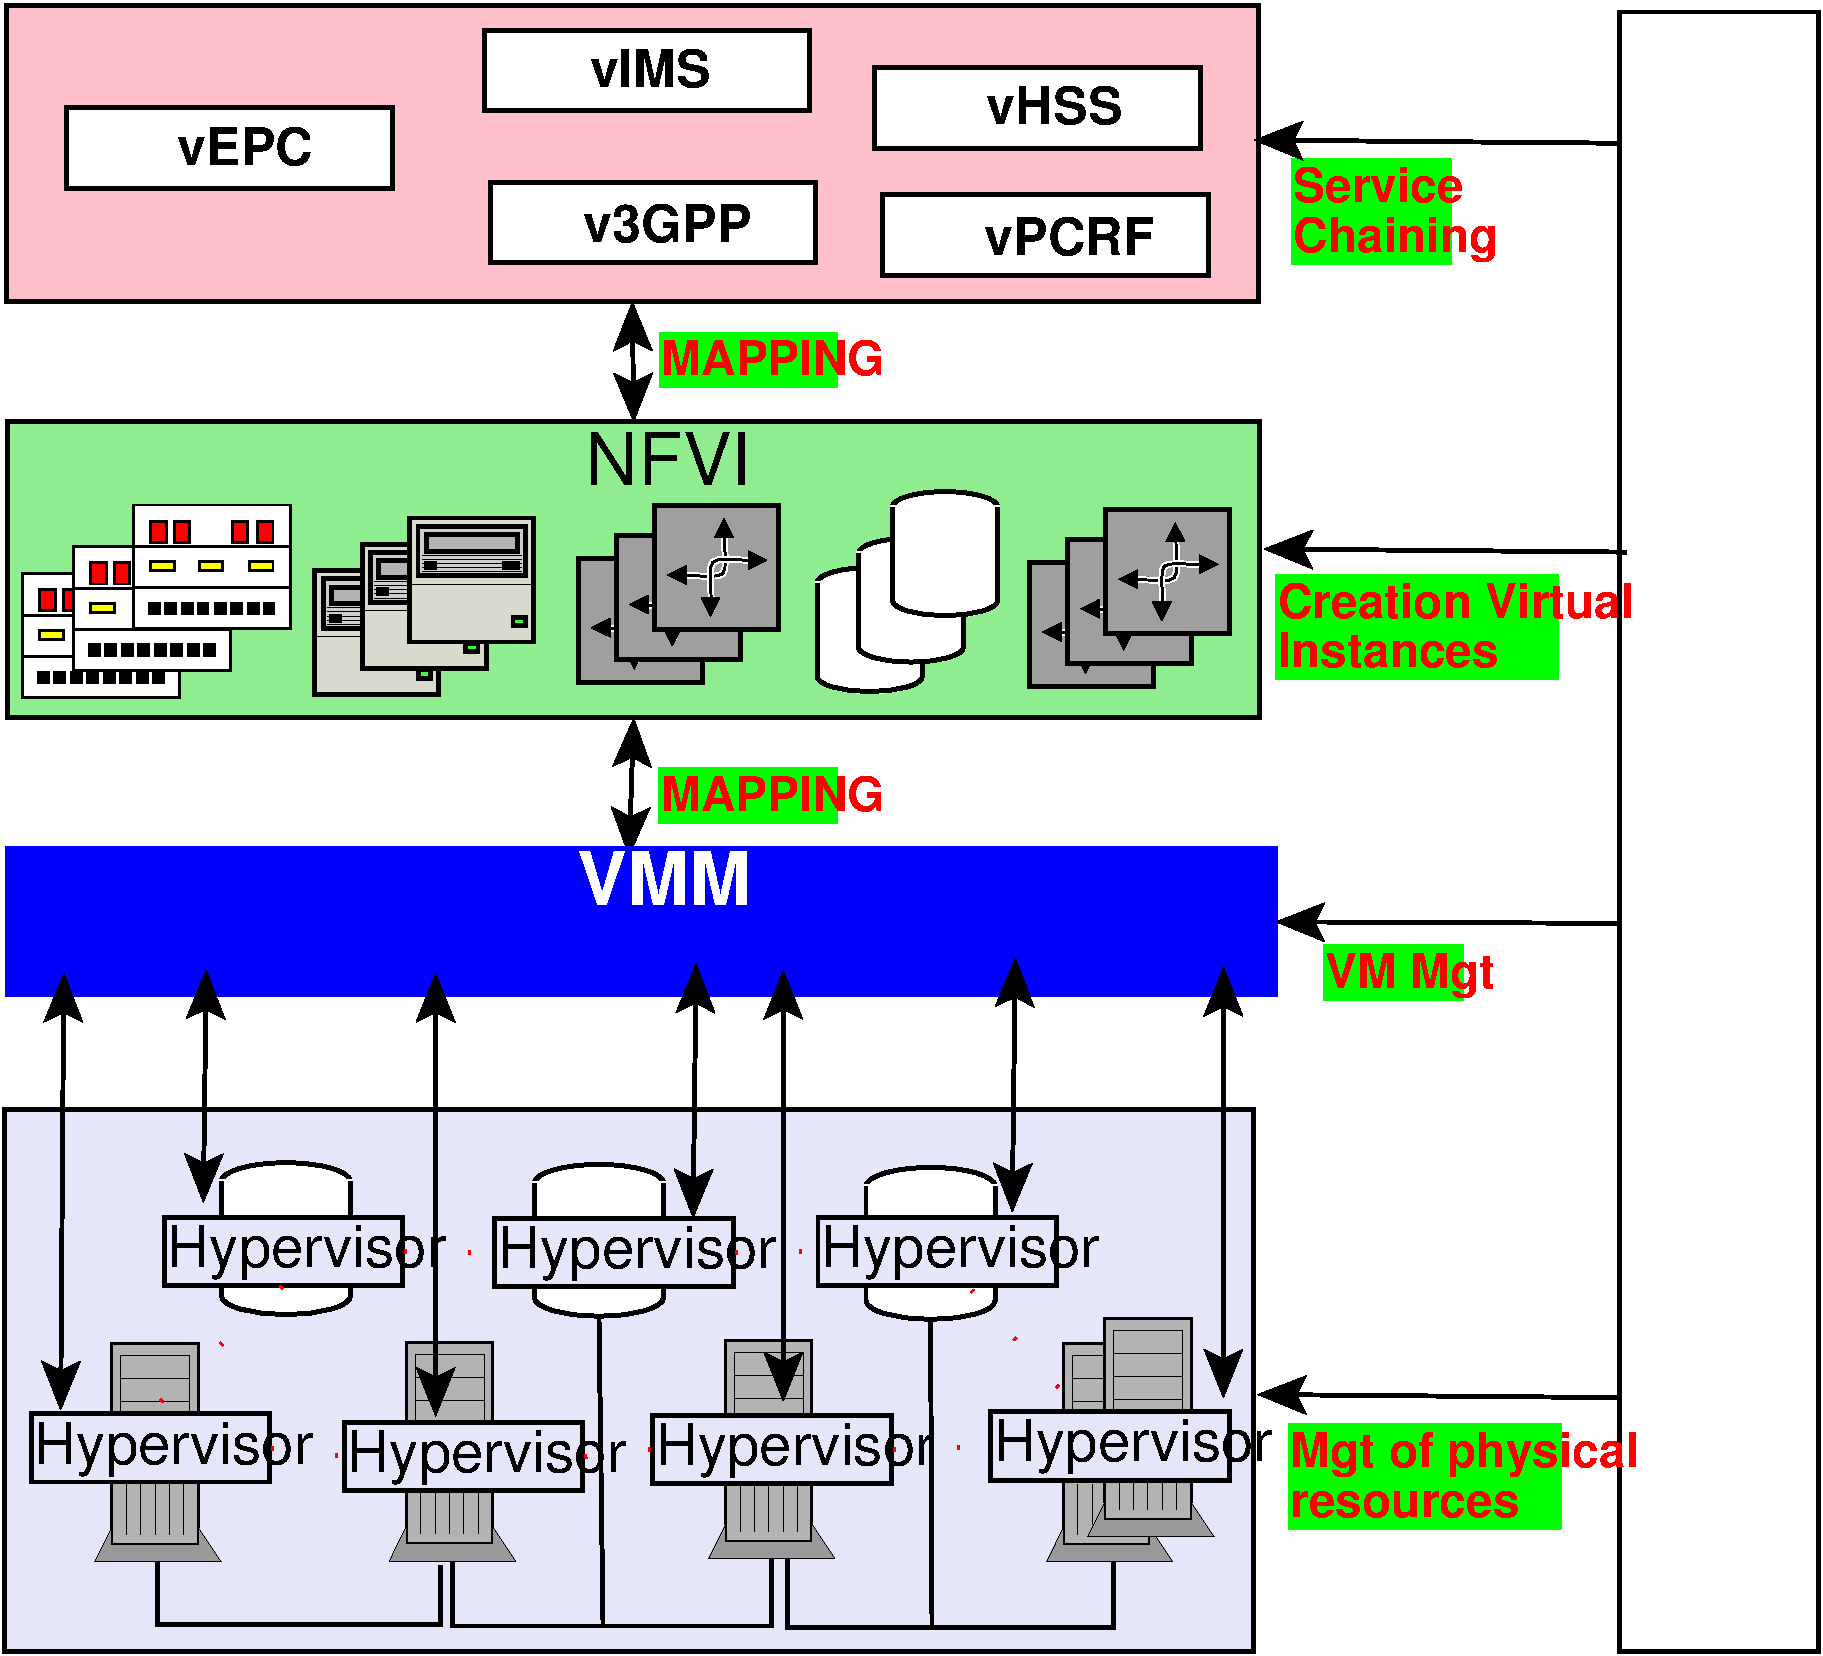
\includegraphics[scale=0.23]{fig/architecture-single.pdf}
	\caption{NFV Reference Architecture}
	\label{fig:arch}
\end{figure} 

In this discussion we use ETSI's NFV architectural model~\cite{nfv} as our main
reference model. Accordingly, the NFV architecture can be classified into three
layers: the first layer is comprised of hardware resources including computing,
storage and network devices, on which physical computing and communication take
place. Typically, this layer is built on computing clusters with
high-performance storage and networking devices. The second layer is
virtualization layer where one or more hypervisors virtualize hardware's
computing, communication and storage capabilities into sharable virtual
resources, some example of hypervisors suitable for such tasks are, KVM, Xen or
VMware, etc. Virtualization layer manages physical resources by means of
scheduling the usage of CPU cycle, network interface virtualization (vNIC) or
block storage devices through a pre-defined virtual infrastructure to hardware
interface (VI-Ha). Having the virtualization resources provisioned, virtual
infrastructures are now managed by platform such as OpenStack~\cite{openstack}
or CloudStack~\cite{cloudstack} for sharing among multiple tenants for service
implementation. A vertial component commonly known as Management and Netowork
Operation (MANO) is supposed to deal with management activities on different
layers and assist users to orchestrate NFV services on the top. 

